\documentclass[a4paper]{article}
\usepackage{url} 
\usepackage{geometry}
\usepackage{graphicx}
\usepackage[parfill]{parskip}
\usepackage{pgfplots}
\usetikzlibrary{external}
\tikzset{external/system call={lualatex \tikzexternalcheckshellescape 
         -enable-write18 -halt-on-error -interaction=nonstopmode 
         -jobname "\image" "\texsource"}}
\tikzexternalize % activate!
\begin{document}
\begin{figure}[ht]
 
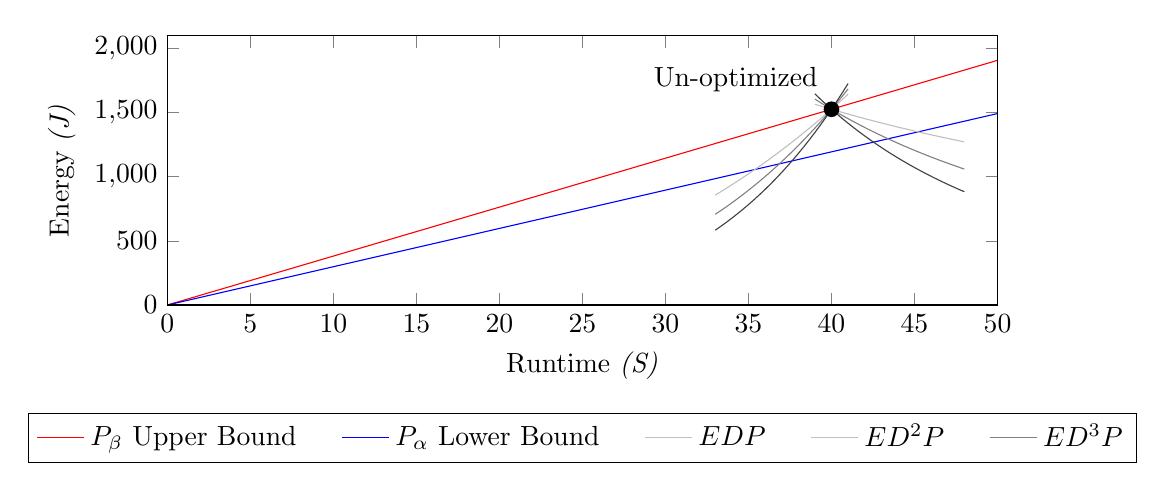
\begin{tikzpicture}
  \begin{axis}[no markers, ylabel={Energy \emph{(J)}}, xlabel={Runtime \emph{(S)}}, axis on top,
    ymin=0,
    xmin=0, xmax=50,
    width=\textwidth,
    height=5cm,
    legend style={at={(0.5,-0.4)}, anchor=north,legend columns=-1, /tikz/every even column/.append style={column sep=0.5cm}}
    ]


     \pgfmathsetmacro{\baseline}{29.857}
     \pgfmathsetmacro{\sedtargetpower}{38.157} % TODO change me
     \pgfmathsetmacro{\sedtargetseconds}{40} % TODO change me
     \pgfmathsetmacro{\sedtargetenergy}{\sedtargetpower * \sedtargetseconds}
 
     \addplot[domain=0:60, red] {\sedtargetpower * x};
     \addlegendentry{$P_{\beta}$ Upper Bound}
     
     \addplot[domain=0:60, blue] {\baseline * x};
     \addlegendentry{$P_{\alpha}$ Lower Bound} 
  
     \addplot[domain=39:48, lightgray] { (\sedtargetenergy * \sedtargetseconds) / ((x))};
     \addplot[domain=33:41, lightgray] { (\sedtargetpower / \sedtargetseconds^2) * x^3}; % Power time same ratio
     \addlegendentry{$EDP$} 
   
     \addplot[domain=39:48, gray] { (\sedtargetenergy * \sedtargetseconds *  \sedtargetseconds) / ((x)^2)};
     \addplot[domain=33:41, gray] { (\sedtargetpower / \sedtargetseconds^3) * x^4}; % Power time same ratio

     \addlegendentry{$ED^{2}P$} 
    
  
     \addplot[domain=39:48, darkgray] { (\sedtargetenergy * \sedtargetseconds * \sedtargetseconds * \sedtargetseconds) / ((x)^3)};
     \addplot[domain=33:41, darkgray] { (\sedtargetpower / \sedtargetseconds^4) * x^5}; % Power time same ratio
     \addlegendentry{$ED^{3}P$} 
    
      
     \node[label={120:{Un-optimized}},circle,fill,inner sep=2pt] at (axis cs:\sedtargetseconds,\sedtargetenergy) {};
 \end{axis}
\end{tikzpicture}
\end{figure}
\end{document}
